% =============================================================================
%  Dinamica3_Fase1_Diapositiva2.tex — Dinámica 3, Fase 1, Diapositiva 2:
%  el filtro del hiperfoco. Mismo pergamino que la Diapositiva 1, con bokeh
%  cálido y sutil, texto secundario difuminado y frases clave nítidas con su
%  traducción.
%  Formato 16:9. Compilar con pdflatex; exportar a PNG con:
%    pdftoppm -png -scale-to-x 1920 -scale-to-y 1080 -singlefile \
%      Dinamica3_Fase1_Diapositiva2.pdf Dinamica3_Fase1_Diapositiva2
% =============================================================================
\documentclass[tikz,border=0pt]{standalone}
\usepackage[utf8]{inputenc}
\usepackage[T1]{fontenc}
\usepackage{ebgaramond}
\usetikzlibrary{fadings}

% ── Parámetros ────────────────────────────────────────────────────────────────
%  \Difuminado: intensidad del desenfoque del texto secundario (0 = nítido,
%  1 = ilegible). Rango sugerido para la dinámica: 0.30 – 0.40.
\def\Difuminado{0.35}
\def\RadioMax{5}        % radio máximo del desenfoque, en pt (con \Difuminado = 1)
\def\TamLetra{26}       % tamaño de letra, en pt
\def\Interlinea{37}     % interlineado, en pt

% ── Paleta (pergamino idéntico a la Diapositiva 1) ────────────────────────────
\definecolor{Pergamino}{HTML}{F1EBDD}
\definecolor{PergaminoBorde}{HTML}{DCCFB4}
\definecolor{Fibra}{HTML}{B9A27A}
\definecolor{Tinta}{HTML}{2B2620}
\definecolor{Resalte}{HTML}{FFE14D}
\definecolor{Traduccion}{HTML}{6B3E12}
\definecolor{BokehDorado}{HTML}{E8B04B}
\definecolor{BokehAmbar}{HTML}{D9893A}
\definecolor{BokehCrema}{HTML}{FFF8E7}

% ── Dimensiones (16:9) ────────────────────────────────────────────────────────
\def\ancho{32}
\def\alto{18}

% ── Marcado del texto ─────────────────────────────────────────────────────────
%  El bloque se dibuja en dos capas con la misma geometría:
%   - capa difusa: solo el texto secundario (las frases clave son \phantom);
%   - capa nítida: solo las frases clave y sus traducciones.
\newif\ifcapanitida
\newcommand{\Sec}[1]{\ifcapanitida\phantom{#1}\else#1\fi}
\newcommand{\Clave}[2]{%
  \ifcapanitida
    \colorbox{Resalte}{\textcolor{Tinta}{#1}}%
    \ \textcolor{Traduccion}{$\rightarrow$\ \textit{(#2)}}%
  \else
    \phantom{\colorbox{Resalte}{#1}\ $\rightarrow$\ \textit{(#2)}}%
  \fi}

\newcommand{\Bloque}{%
  \Sec{Mas luego que a la tierra llegamos, que estaba vecina,}\\
  \Clave{vimos en un extremo una cueva}{Encuentran una guarida}\\
  \Sec{alta y techada de lauros; allí se albergaban rebaños}\\
  \Sec{copiosos de ovejas y cabras, y en torno un recinto}\\
  \Sec{se alzaba, de piedras hundidas y recias encinas.}\\
  \Clave{Allí pernoctaba un varón monstruoso}{Hay un habitante hostil}\\
  \Sec{que apacentaba sus ganados muy lejos, y con nadie se congregaba,}\\
  \Sec{sino que, apartado, vivía en la profunda iniquidad.}\\
  \Sec{Era un monstruo gigante, y en nada se asemejaba}\\
  \Sec{a los hombres que comen pan,} \Clave{sino a un pico silvestre.}{No es humano, es gigante}%
}

\begin{document}
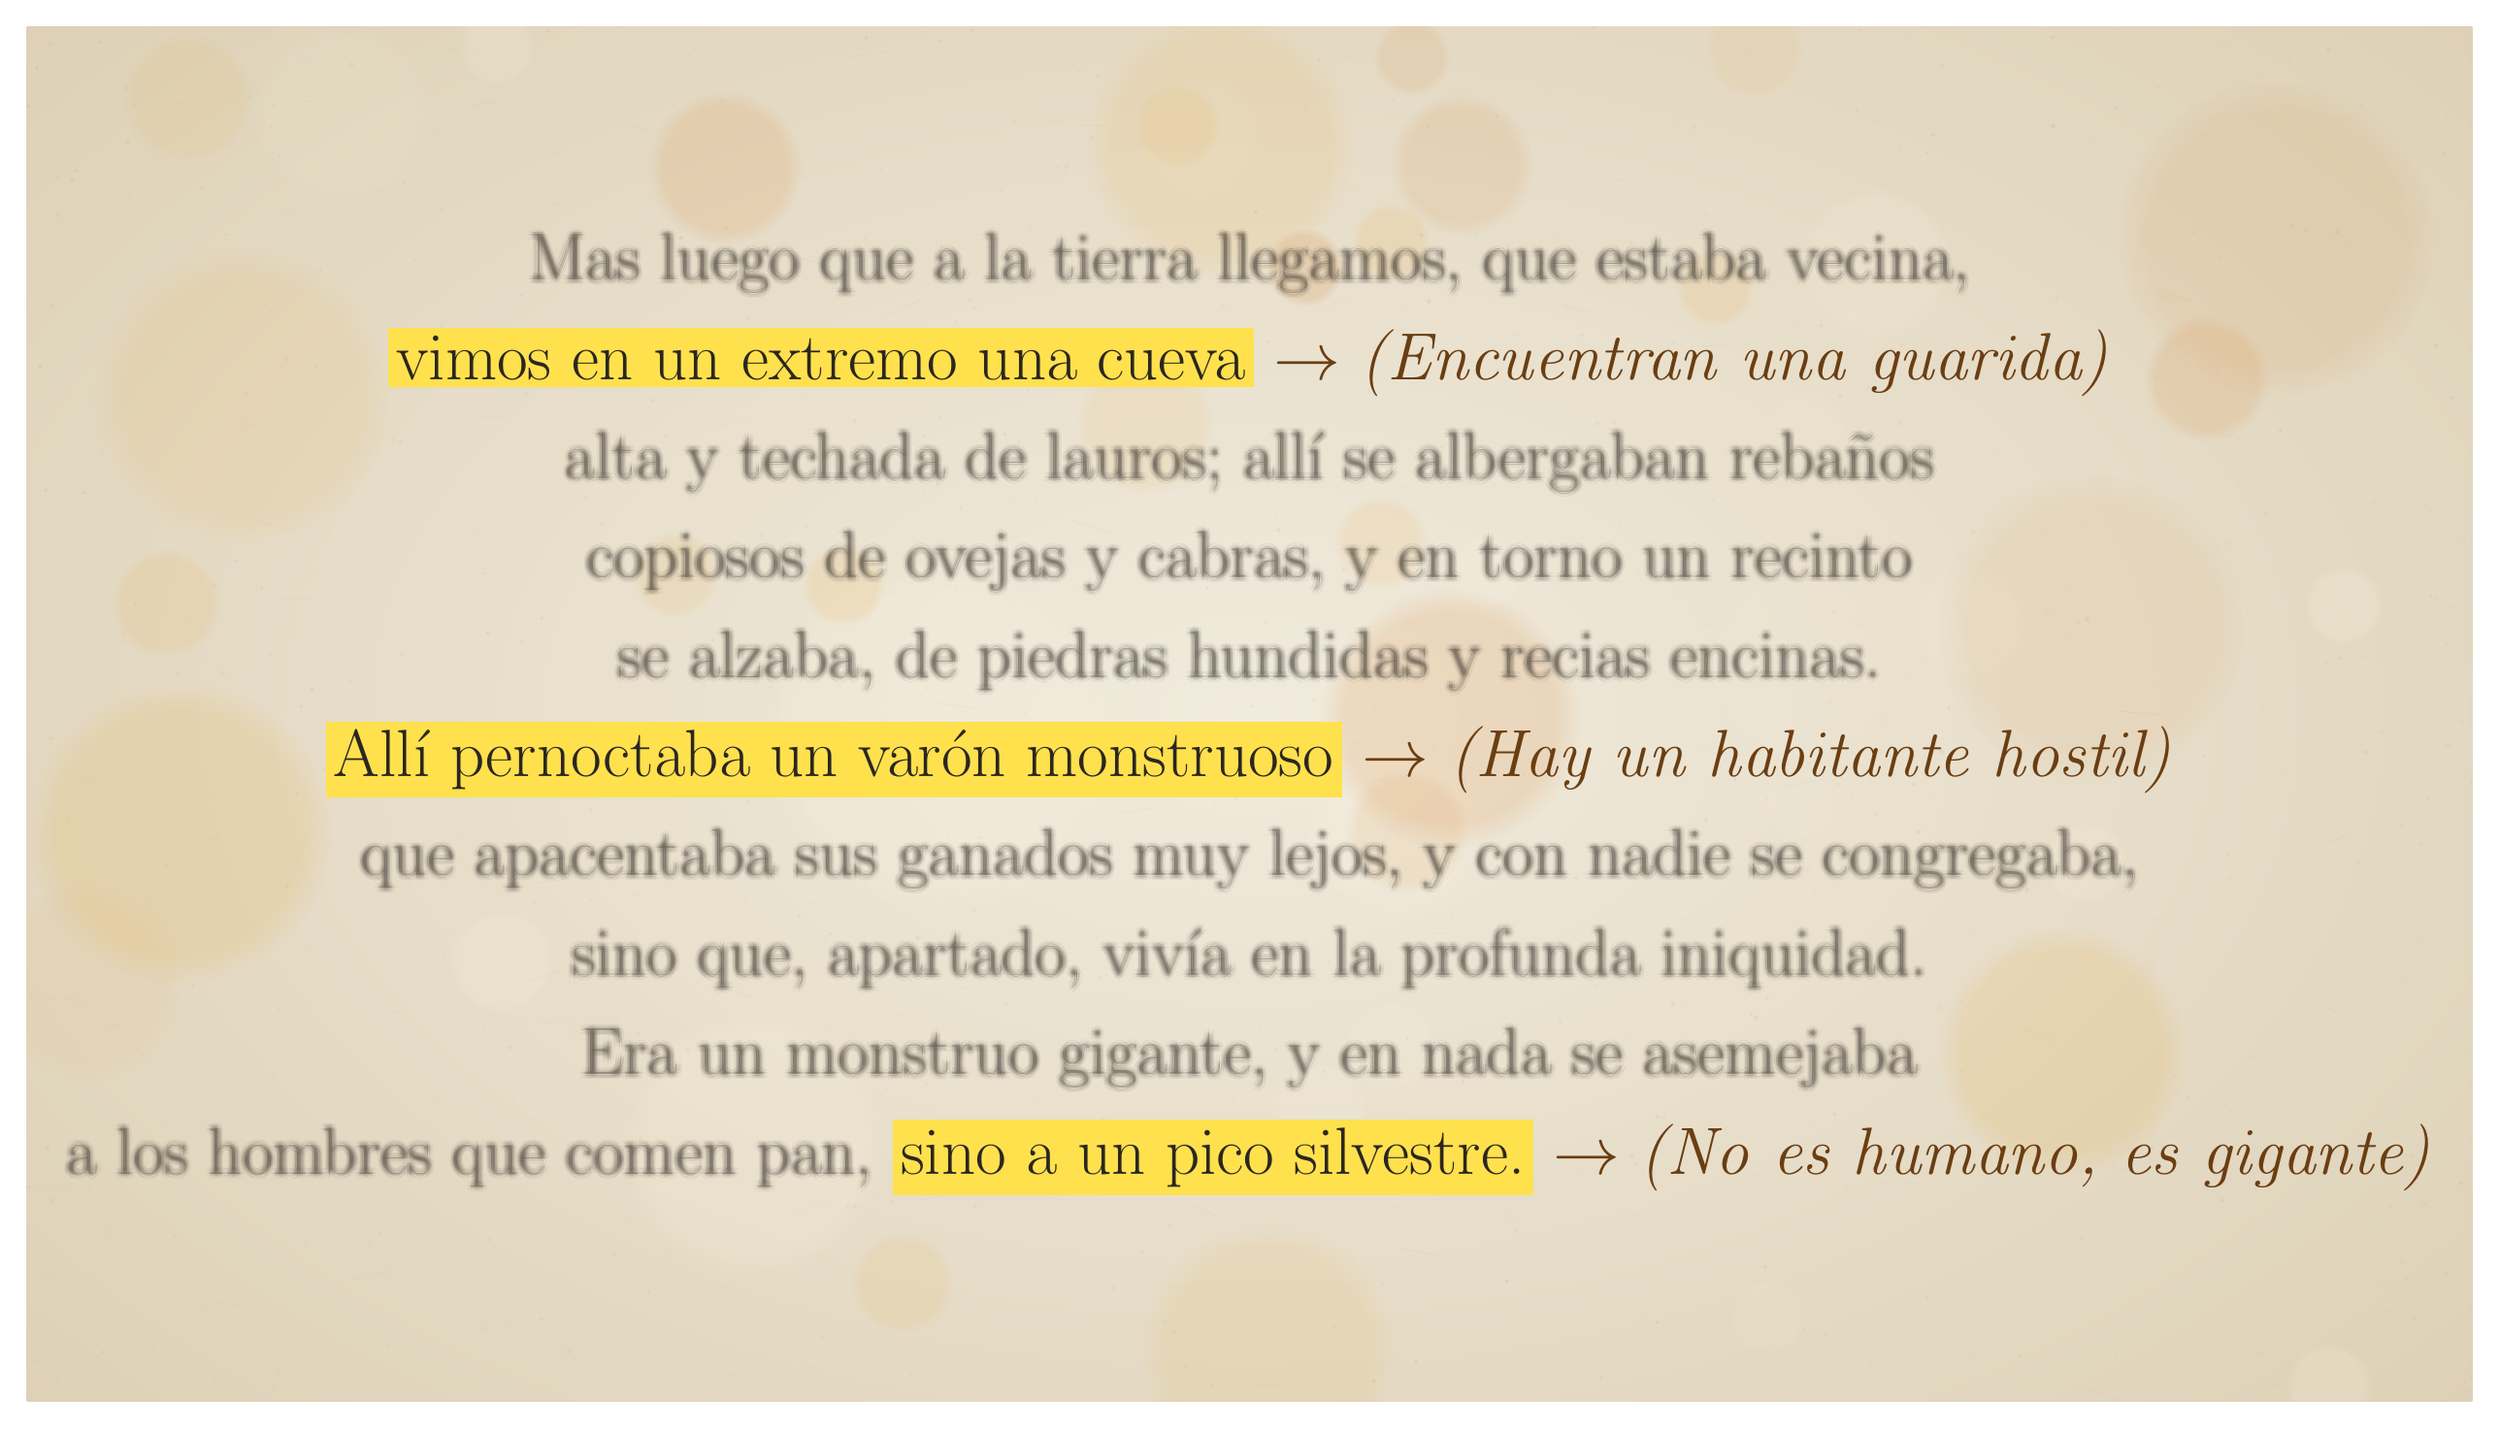
\begin{tikzpicture}
  % Área fija 16:9: nada se dibuja fuera de ella
  \useasboundingbox (0,0) rectangle (\ancho,\alto);
  \clip (0,0) rectangle (\ancho,\alto);

  % Fondo con viñeta (igual que la Diapositiva 1)
  \fill[PergaminoBorde] (0,0) rectangle (\ancho,\alto);
  \shade[inner color=Pergamino, outer color=PergaminoBorde]
    (\ancho/2,\alto/2) ellipse [x radius=0.72*\ancho, y radius=0.80*\alto];

  % Textura: fibras y motas finas (misma semilla que la Diapositiva 1)
  \pgfmathsetseed{1914}
  \foreach \i in {1,...,900}{
    \pgfmathsetmacro{\x}{rnd*\ancho}
    \pgfmathsetmacro{\y}{rnd*\alto}
    \pgfmathsetmacro{\r}{0.008+0.02*rnd}
    \pgfmathsetmacro{\o}{0.05+0.12*rnd}
    \fill[Fibra, opacity=\o] (\x,\y) circle (\r);
  }
  \foreach \i in {1,...,140}{
    \pgfmathsetmacro{\x}{rnd*\ancho}
    \pgfmathsetmacro{\y}{rnd*\alto}
    \pgfmathsetmacro{\l}{0.15+0.5*rnd}
    \pgfmathsetmacro{\a}{-25+50*rnd}
    \pgfmathsetmacro{\o}{0.04+0.08*rnd}
    \draw[Fibra, opacity=\o, line width=0.25pt, rotate around={\a:(\x,\y)}]
      (\x,\y) -- ++(\l,0);
  }

  % Bokeh cálido y sutil sobre el pergamino (semilla fija)
  \pgfmathsetseed{2026}
  \foreach \i in {1,...,45}{
    \pgfmathsetmacro{\x}{rnd*\ancho}
    \pgfmathsetmacro{\y}{rnd*\alto}
    \pgfmathsetmacro{\r}{0.5+1.9*rnd^2}
    \pgfmathsetmacro{\o}{0.06+0.12*rnd}
    \pgfmathtruncatemacro{\c}{int(3*rnd)}
    \ifcase\c\relax \def\col{BokehDorado}\or \def\col{BokehAmbar}%
      \else \def\col{BokehCrema}\fi
    \fill[\col, fill opacity=\o, path fading=circle with fuzzy edge 20 percent]
      (\x,\y) circle (\r);
  }

  % Estilo común del bloque de texto
  \tikzset{bloque/.style={anchor=center, align=center, inner sep=0pt,
    font=\fontsize{\TamLetra}{\Interlinea}\selectfont}}
  \coordinate (centro) at (\ancho/2,\alto/2);

  % Capa difusa: el texto secundario se dibuja varias veces con pequeños
  % desplazamientos en dos anillos y opacidad baja (desenfoque simulado)
  \pgfmathsetmacro{\R}{\Difuminado*\RadioMax}
  \capanitidafalse
  \foreach \ang in {0,45,...,315}{
    \foreach \f/\op in {1/0.05, 0.5/0.07}{
      \node[bloque, text=Tinta, text opacity=\op]
        at ([shift={(\ang:\f*\R pt)}]centro) {\Bloque};
    }
  }
  \node[bloque, text=Tinta, text opacity={0.35*(1-\Difuminado)}]
    at (centro) {\Bloque};

  % Capa nítida: frases clave resaltadas y traducciones
  \capanitidatrue
  \node[bloque] at (centro) {\Bloque};
\end{tikzpicture}
\end{document}
